\documentclass[12pt]{article}
\usepackage[spanish,mexico]{babel}
\selectlanguage{spanish}
\usepackage{graphicx}
\usepackage{amsmath}
\usepackage{wrapfig}
\usepackage[dvipsnames]{xcolor}
\usepackage{float}
\usepackage{multicol}
\usepackage{geometry}
\usepackage{hyperref}
\usepackage[utf8]{inputenc}

\title{Actividad 9: Aproximación al cálculo del periodo del péndulo}
\author{Paulina Valenzuela Coronado}
\date{Mayo de 2016}

\begin{document}
\maketitle

\section{Introducción}
Un zombie es la representación de un cadáver que de una u otra manera puede resucitar o volver a la vida. Muchas de las diferentes relaciones que se muestran con uno de ellos es una figura legendaria propia del culto vudú. Se trata de un muerto resucitado por medios mágicos por un hechicero para convertirlo en su esclavo. De acuerdo con la creencia, un houngan, bokor o hechicero vudú, sería capaz, mediante un ritual, de resucitar a un muerto, que quedaría, sin embargo, sometido en adelante a la voluntad de la persona que le devuelve la vida. También, según una creencia popular, se dice que una persona que es mordida por un zombi, se convierte en zombi.\cite{U}

\section{¿Qué pasaría si el virus del zombie se diseminara en una población?}
Para entender los modelos el artículo  tiene la siguiente clasificación:
\begin{itemize}
	\item \textbf{S}: Población suceptible a infectarse o morir, vivos.
	\item \textbf{Z}: Población de Zombies.
	\item \textbf{R}: Población de individuos eliminados.
	\item \textbf{I}: Población de infectados.
	\item \textbf{Q}: Población en Cuarentena.
\end{itemize}

En el artículo presentan varios modelos sobre las diferentes situaciones que se presentarían en caso que el virus del zombie se diseminara.

\subsection{Modelo Básico}
En este modelo solamente los sanos \textbf{S} pueden convertirse en zombies \textit{$\beta$} pero pueden evitarlo mediante enfrentamientos \textit{$\alpha$}, pero los muertos pueden volverse zombies aumentando \textbf{Z}
provocando así que \textbf{S} pierda los enfrentamientos.

\begin{figure}[H]
	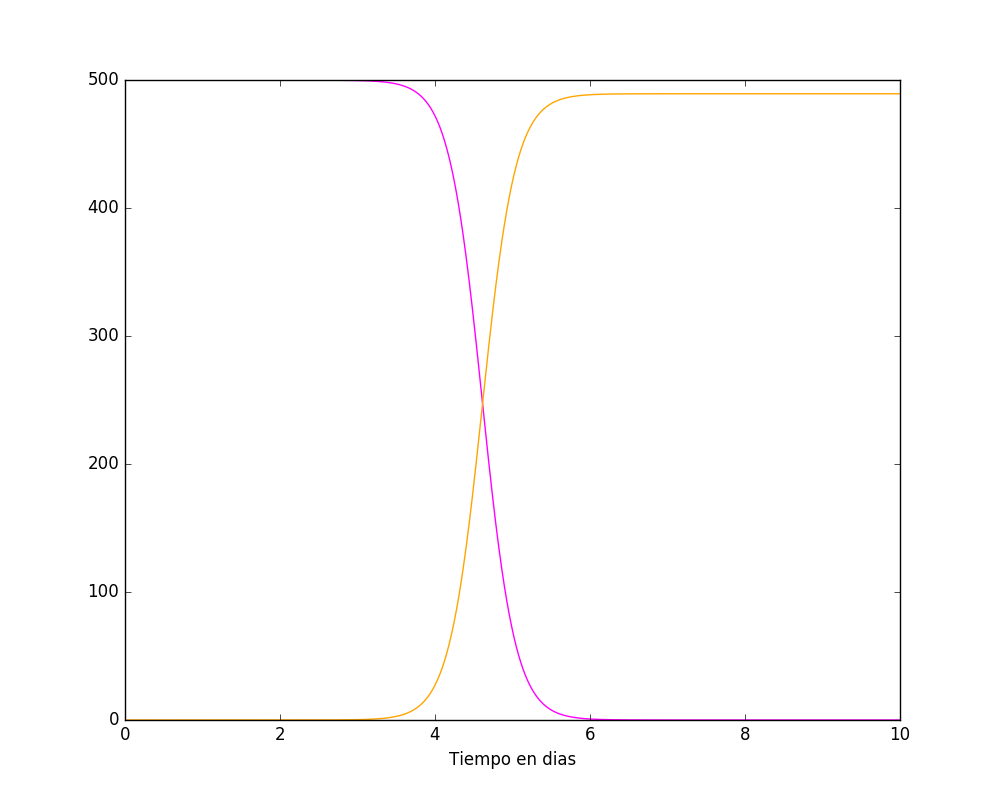
\includegraphics[width=9cm]{basico.png}
\end{figure}

\begin{verbatim}
# -*- coding: utf-8 -*-
# zombie apocalypse modeling
import numpy as np
import matplotlib.pyplot as plt
from scipy.integrate import odeint
plt.ion()
plt.rcParams['figure.figsize'] = 10, 8

P = 0           # birth rate
d = 0.0001  # natural death percent (per day)
B = 0.0095  # transmission percent  (per day)
G = 0.0001  # resurect percent (per day)
A = 0.0002  # destroy percent  (per day)

# solve the system dy/dt = f(y, t)
def f(y, t):
Si = y[0]
Zi = y[1]
Ri = y[2]
# the model equations (see Munz et al. 2009)
f0 = P - B*Si*Zi - d*Si
f1 = B*Si*Zi + G*Ri - A*Si*Zi
f2 = d*Si + A*Si*Zi - G*Ri
return [f0, f1, f2]

# initial conditions
S0 = 500.                   # initial population
Z0 = 0                      # initial zombie population
R0 = 0                      # initial death population
y0 = [S0, Z0, R0]   # initial condition vector
t  = np.linspace(0, 10., 1000)       # time grid

# solve the DEs
soln = odeint(f, y0, t)
S = soln[:, 0]
Z = soln[:, 1]
R = soln[:, 2]

# plot results
plt.figure()
plt.plot(t, S, 'magenta', label='Vivos')
plt.plot(t, Z, 'orange', label='Zombies')
plt.xlabel('Tiempo en dias')
plt.ylabel('Población')
plt.title('Modelo basico')
plt.legend(loc=0)

\end{verbatim}




\subsection{Modelo con Infección Latente}
Este modelo incluye el efecto de una clase de individuos afectados, considerando un tiempo de incubación y efectos del virus en una individuo infectado se crea una tasa de conversión de individuos sanos en zombies, esto modifica a la población \textbf{Z} directamente y retarda el tiempo en el cual \textbf{Z} sobre pasa a \textbf{S} considerablemente.

\begin{figure}[H]
	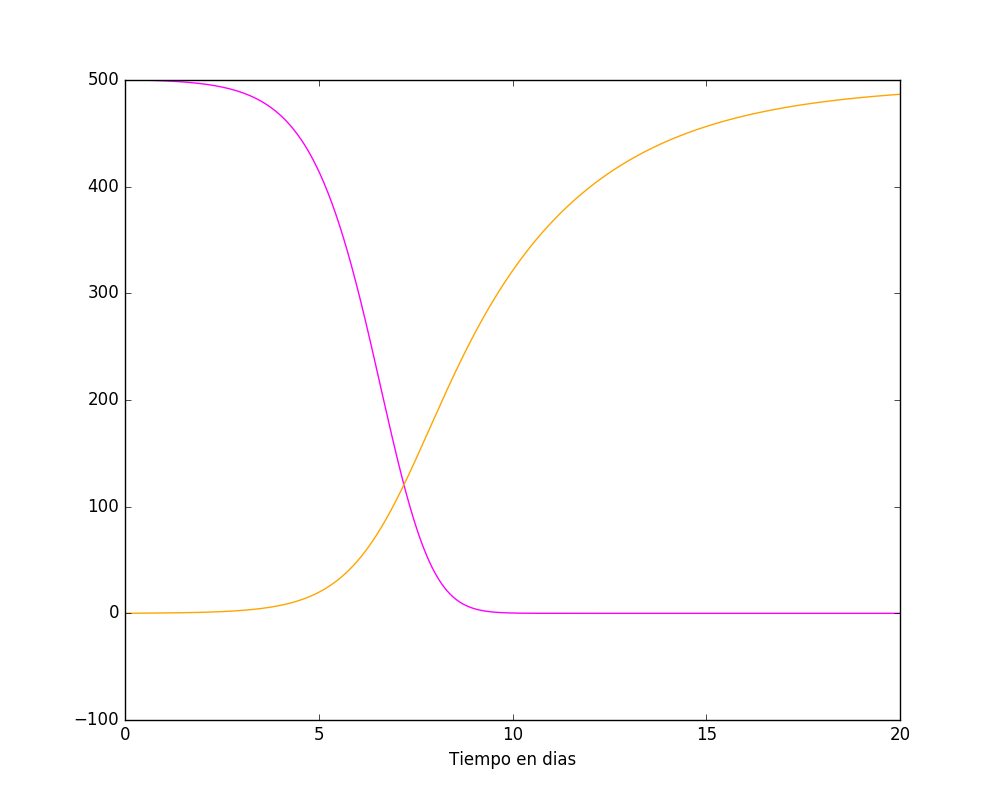
\includegraphics[width=9cm]{infeccion.png}
\end{figure}

\begin{verbatim}
# coding: utf-8

# In[1]:

# Modelo con Infeccion Latente.
import numpy as np
import matplotlib.pyplot as plt
from scipy.integrate import odeint
plt.ion()
plt.rcParams['figure.figsize'] = 10, 8

P = 0           # birth rate
d = 0.0001  # natural death percent (per day)
B = 0.0095  # transmission percent  (per day)
G = 0.0001  # resurect percent (per day)
A = 0.0001  # destroy percent  (per day)
rho = 0.3

# solve the system dy/dt = f(y, t)
def f(y, t):
Si = y[0]
Ii = y[1]
Zi = y[2]
Ri = y[3]

# the model equations (see Munz et al. 2009)
f0 = P - B*Si*Zi - d*Si
f1 = B*Si*Zi - rho*Ii - d*Ii
f2 = rho*Ii + G*Ri - A*Si*Zi
f3 = d*Si + d*Ii + A*Si*Zi - G*Ri
return [f0, f1, f2, f3]

# initial conditions
S0 = 500                   # initial population
I0 = 1
Z0 = 0                      # initial zombie population
R0 = 0                      # initial death population

y0 = [S0, I0, Z0, R0]   # initial condition vector
t  = np.linspace(0, 20, 1000)       # time grid

# solve the DEs
soln = odeint(f, y0, t)
S = soln[:, 0]
I = soln[:, 1]
Z = soln[:, 2]
R = soln[:, 3]


# plot results
plt.figure()
plt.plot(t, S, 'magenta', label='Vivos')
plt.plot(t, Z, 'orange', label='Zombies')
plt.xlabel('Tiempo en dias')
plt.ylabel('Población')
plt.title('Modelo con Infeccion Latente')
plt.legend(loc=0)
\end{verbatim}

\subsection{Modelo con Cuarentena}
En este modelo, se busca contener el brote del virus, así que la población decide aislar a los infectados en cuarentena pero también a una cierta cantidad de zombies para ver si ellos también pueden llegar a curarse. Pero los individuos en cuarentena pueden tratar de escapar y deben de ser eliminados o podrían morir estando en la cuarentena.

\begin{figure}[H]
	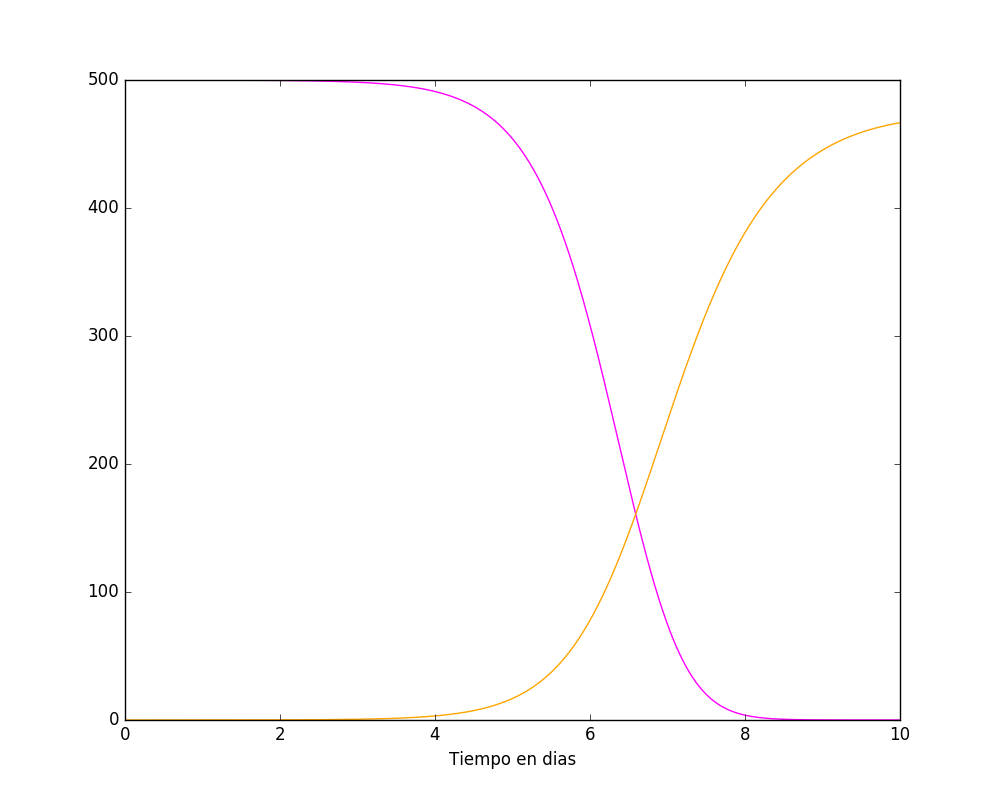
\includegraphics[width=9cm]{cuarentena.png}
\end{figure}



\begin{verbatim}
# -*- coding: utf-8 -*-
# zombie apocalypse modeling
import numpy as np
import matplotlib.pyplot as plt
from scipy.integrate import odeint
plt.ion()
plt.rcParams['figure.figsize'] = 10, 8

P = 0           # birth rate
d = 0.0001  # natural death percent (per day)
B = 0.0095  # transmission percent  (per day)
G = 0.0001  # resurect percent (per day)
A = 0.0001  # destroy percent  (per day)
rho=1  # parámetro que no conozco
k=0.001
sigma=0.009
Ga=0.004

#0.0000475

# solve the system dy/dt = f(y, t)
def f(y, t):
Si = y[0]
Ii = y[1]
Zi = y[2]
Ri = y[3]
Qi = y[4]
# the model equations (see Munz et al. 2009)
f0 = P - B*Si*Zi - d*Si
f1 = (B*Si*Zi)-(rho*Ii)-(d*Ii)-(k*Ii)
f2 = (rho*Ii) + (G*Ri)-(A*Si*Zi)-(sigma*Zi)
f3 = (d*Si) + (d*Ii) + (A*Si*Zi)-(G*Ri)+(Ga*Qi)
f4 = (k*Ii)+(sigma*Zi)-(Ga*Qi)

return [f0, f1, f2, f3, f4]

# initial conditions
S0 = 500.                   # initial population
Z0 = 0.                      # initial zombie population
R0 = 0.                      # initial death population
I0 = 100.
Q0 = 130.
y0 = [S0, Z0, R0, I0, Q0]   # initial condition vector
t  = np.linspace(0, 10., 1000)       # time grid

# solve the DEs
soln = odeint(f, y0, t)
S = soln[:, 0]
I = soln[:, 1]
Z = soln[:, 2]
R = soln[:, 3]
Q = soln[:, 4]

# plot results
plt.figure()
plt.plot(t, S, 'magenta', label='Vivos')
plt.plot(t, Z, 'orange', label='Zombies')
plt.xlabel('Tiempo en dias')
plt.ylabel('Población')
plt.title('Modelo con Cuarentena')
plt.legend(loc=0)
\end{verbatim}
\subsection{Modelo con Tratamiento/Cura}
En este modelo se supone que se puede curar a los zombies permitiendoles volver a ser humanos, de esta manera se elimina la necesidad de tener en cuarentena a todos, pero los individuos salvados ahora vuelven a ser suceptibles y forman parte de \textbf{S}. 

\begin{figure}[H]
	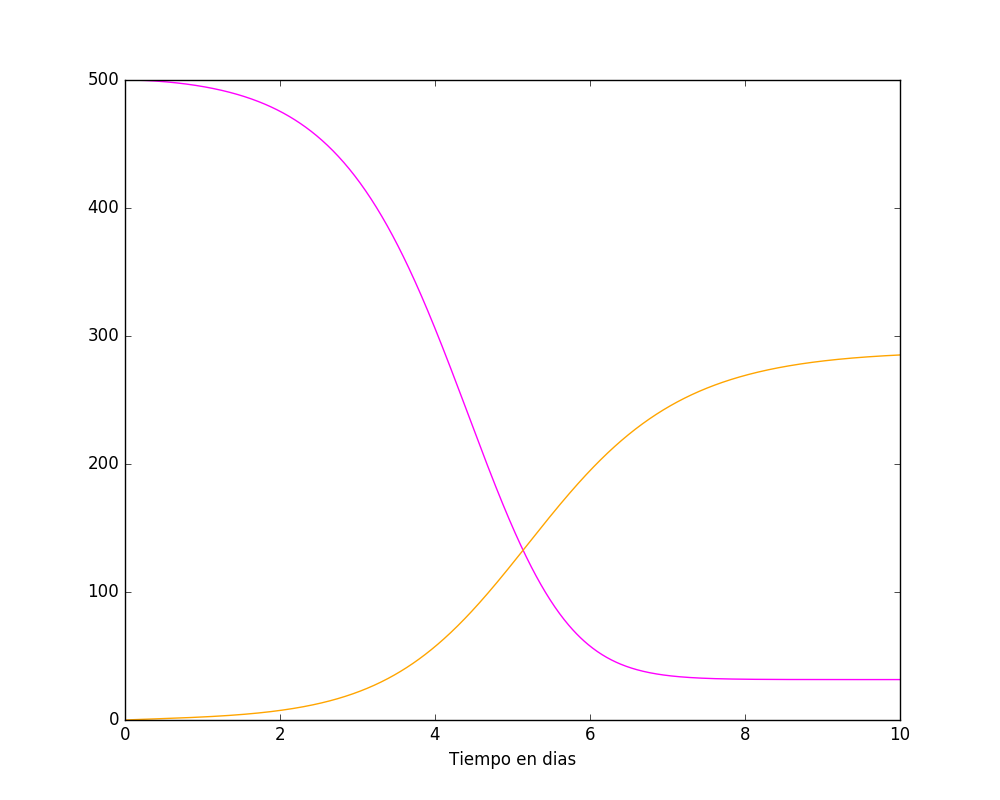
\includegraphics[width=9cm]{tratamiento.png}
\end{figure}





\begin{verbatim}
# coding: utf-8

# In[15]:

# Modelo con Infeccion Latente.
import numpy as np
import matplotlib.pyplot as plt
from scipy.integrate import odeint
plt.ion()
plt.rcParams['figure.figsize'] = 10, 8

P = 0           # birth rate
d = 0.0001  # natural death percent (per day)
B = 0.0095  # transmission percent  (per day)
G = 0.0001  # resurect percent (per day)
A = 0.0001  # destroy percent  (per day)
rho = 0.5
c = 0.3

# solve the system dy/dt = f(y, t)
def f(y, t):
Si = y[0]
Ii = y[1]
Zi = y[2]
Ri = y[3]

# the model equations (see Munz et al. 2009)
f0 = P - B*Si*Zi - d*Si + c*Zi
f1 = B*Si*Zi - rho*Ii - d*Ii
f2 = rho*Ii + G*Ri - A*Si*Zi - c*Zi
f3 = d*Si + d*Ii + A*Si*Zi - G*Ri
return [f0, f1, f2, f3]

# initial conditions
S0 = 500                   # initial population
I0 = 5
Z0 = 0                      # initial zombie population
R0 = 0                      # initial death population

y0 = [S0, I0, Z0, R0]   # initial condition vector
t  = np.linspace(0, 10, 1000)       # time grid

# solve the DEs
soln = odeint(f, y0, t)
S = soln[:, 0]
I = soln[:, 1]
Z = soln[:, 2]
R = soln[:, 3]


# plot results
plt.figure()
plt.plot(t, S, 'magenta', label='Vivos')
plt.plot(t, Z, 'orange', label='Zombies')
plt.xlabel('Tiempo en dias')
plt.ylabel('Población')
plt.title('Modelo con Tratamiento')
plt.legend(loc=0)
\end{verbatim}
\
\begin{thebibliography}{6}
	
	\bibitem{P}
	\emph{Zombiepedia}. 
	\url{http://zombie.wikia.com/wiki/Zombie_Wiki}
	
	
	\bibitem{A}
	\emph{Artículo}
	\url{http://mysite.science.uottawa.ca/rsmith43/Zombies.pdf}
		
		
	\bibitem{U}
	\emph{Zombie}. 
	\url{https://es.wikipedia.org/wiki/Zombi}	
	\end{thebibliography}

\end{document}